\section{Comparaison avec la photo avec une légère
rotation}\label{comparaison-avec-la-photo-avec-une-luxe9guxe8re-rotation}

\begin{figure}[htbp]
\centering
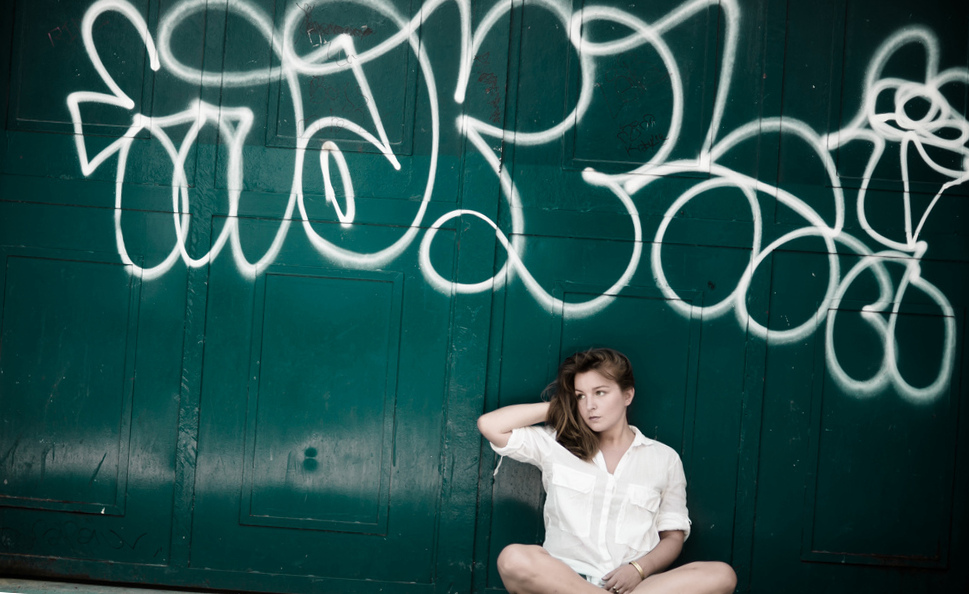
\includegraphics{../../photos/rotate.jpg}
\caption{Photo rotation légère}
\end{figure}

\begin{table}[htbp]
\centering
\begin{tabular}{llr}
\bfseries Formes &
\bfseries Bhattacharyya (\%)%
\DTLforeach*[\DTLiseq{\fichier}{photos/rotate.jpg}]{valeurs}{%
\fichier=Fichier, \formes=Formes,\bhatta=Bhattacharyya, \hue=Hue, \saturation=Saturation, \value=Value}{%
\\
\formes & \bhatta}
\end{tabular}
\end{table}


Pour cette comparaison, on observe une très faible différence de
couleurs (seulement $0.64 \%$), car l'text = Image est seulement retournée donc
les couleurs ne changent quasiment pas. Par contre la différence de
formes est assez élevée car tous les pixels sont décalés ($53.58 \%$ de
différence après application du filtre de Sobel).\\On constate donc que
la rotation légère ne change pas beaucoup les couleurs de la photo mais
majoritairement ses formes.